\documentclass{article}

\usepackage[utf8]{inputenc}
\usepackage{amsthm}
\usepackage{amssymb}
\usepackage{amsfonts}
\usepackage[francais]{babel}
\usepackage{fancyvrb}
\usepackage{hyperref}
\usepackage{graphicx}

 
\author{Ye Daniel, Kouadri Amine.} 


\title{Compte rendu du tp2}


\begin{document}

\maketitle
Voici les réponses aux questions du tp:

\paragraph{question 1.b:}
~~\\
représentation graphique de la fonction $f(x) = \sqrt{1 - x^2}$ \\
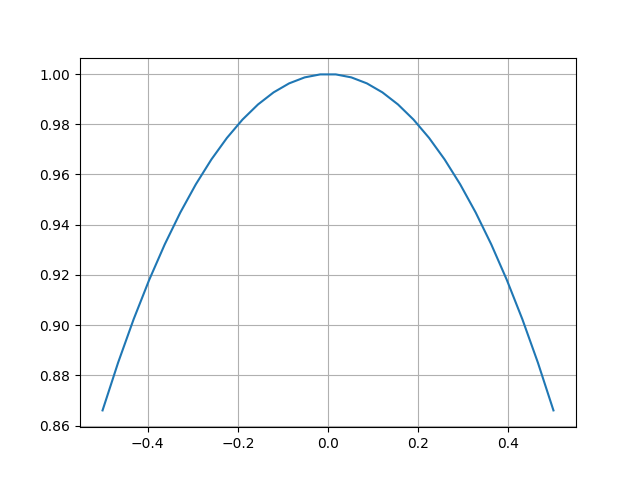
\includegraphics[height=5cm]{f.png}
\paragraph{question 1.c:}
~~\\
$\int_{-0.5}^{0.5} f(x) \, \mathrm dx= [\frac{1}{2}(x \sqrt{1-x^2}+\arcsin(x)]_{-0.5}^{0.5}$
\\
$\int_{-0.5}^{0.5}f(x)\mathrm dx\approx0.956$
\paragraph{question 2.c:}
~~\\
Méthode du point milieu:
\\
l'aire du rectangle pour chaque subdivision est notée $s_i$:
\\
$s_1=\sqrt{\frac{3}{2}}\times{0.25}$, 
$s_2=\frac{\sqrt{15}}{4}\times{0.25}$,
$s_3=\frac{\sqrt{15}}{4}\times{0.25}$,
$s_4=\sqrt{\frac{3}{2}}\times{0.25}$.
\\ 
\\
$s_1\approx0.22$,
$s_2\approx0.24$,
$s_3\approx0.24$,
$s_4\approx0.22$.
\\
\\
La somme totale des aires des rectangles est $S\approx0.9171$
\\ \\
L'erreur commise est égale à 0.04.
\\
\paragraph{question 2.f}:
~~\\
L'erreur commise pour chaque pas $p=\frac{1}{n}$ avec n=$10^k,$ k variant de 1 à 6:
\\
\VerbatimInput{tableau_point_milieu.txt}
\paragraph{question 4}
~~\\
Méthode du trapèze:
\\
soit p=$\frac{(b-a)}{n}$ le pas choisi, et $T_i$ l'aire de chaque trapèze on a:
\\ \\
$T_i=\frac{(f(a+p\times{i})+ f(a+p\times{(i+1)}))\times{p}}{2}$
\\ \\
$\int_{a}^{b}f(x)\mathrm dx \approx \sum_{i=1}^{n} T_i$
\\
\\
L'erreur commise pour a=-0.5, b=0.5, pour chaque pas $p=\frac{1}{n}$ avec n=$10^k,$ k variant de 1 à 6:
\\
\VerbatimInput{tableau_trapeze.txt}
Méthode de Simpson:
\\ \\
soit n le nombre d'intervalles de [a,b], et h=$\frac{(b-a)}{n}$ la longueur de ces intervalles, et $x_i$=a+ih pour {i=0,1,...,n-1,n.} on a:
\\
$\int_{a}^{b}f(x)\mathrm dx \approx (\frac{h}{3})[f(a)+ 2 \sum_{i=1}^{\frac{n}{2}-1} f(x_{2i})+4 \sum_{i=1}^{\frac{n}{2}} f(x_{2i-1}) + f(x_n)]$
\\ \\
l'erreur commise pour a=-0.5, b=0.5 avec n=$10^k, k$ variant de 1 à 6.
\\
\VerbatimInput{tableau_simpson.txt}
\paragraph{question 5}:
~~\\
Les méthodes de Simpson et du Trapèze sont plus précises, la méthode du point milieu est plus rapide.
\paragraph{question 6.c}:
~~\\
représentation du cercle unité et génération aléatoire de points dont les deux coordonnées sont comprises entre -1 et 1.
\\
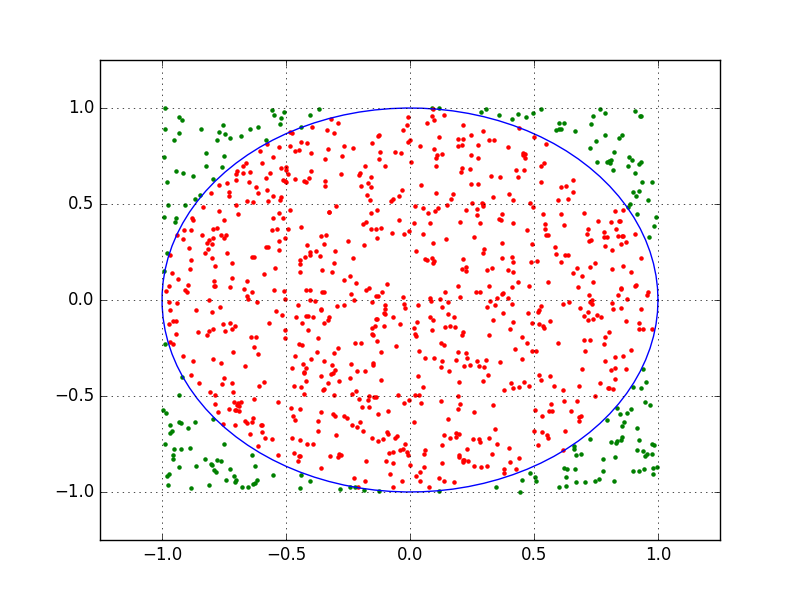
\includegraphics[height=5cm]{cercle.png}
\paragraph{question 6.d}:
~~\\
Méthode de Monte-Carlo:
\\ \\
On a $\frac{I}{N}= \frac{S}{4}$ où I est le nombre de points à l'intérieur du cercle unité, N le nombre de points total et S la valeur de la surface recherchée.
\\
Après calcul l'erreur commise est de 4.840572387e-13 avec un temps de calcul de 3.620000e-04  secondes
\paragraph{question 6.f}
~~\\
Voici l'erreur commise avec la méthode de Monte-Carlo et le temps de calcul avec N=$10^k$, k variant de 1 à 6. 
\\
\VerbatimInput{monte_carlo_cercle.txt}
\newpage
\paragraph{question 6.g}
~~\\
Voici la représentation de la boule unité avec génération aléatoire de points dont touts les coordonnées sont comprises entre -1 et 1.
\\
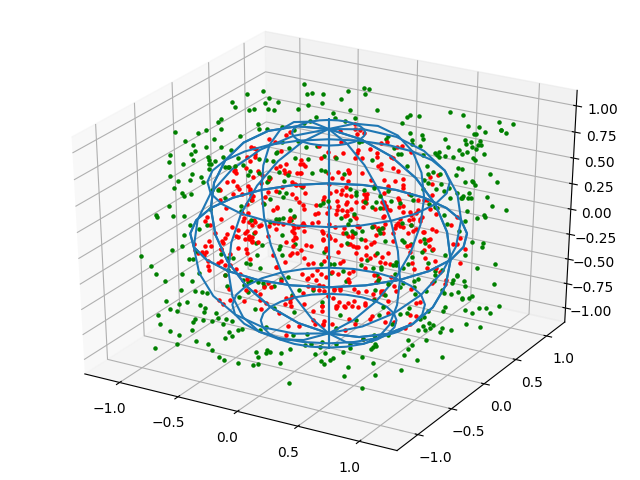
\includegraphics[height=8cm]{sphere.png}
\\
Voici l'erreur commise avec la méthode de Monte-Carlo et le temps de calcul avec  N=$10^k$, k variant de 1 à 6. 
\\
\VerbatimInput{monte_carlo_sphere.txt}
\end{document}
